% !TeX spellcheck = en_GB
%%%%%%%%%%%%%%%%%%%%%%%%%%%%%%%%%%%%%%%%%
% University/School Laboratory Report
% LaTeX Template
% Version 3.1 (25/3/14)
%
% This template has been downloaded from:
% http://www.LaTeXTemplates.com
%
% Original author:
% Linux and Unix Users Group at Virginia Tech Wiki 
% (https://vtluug.org/wiki/Example_LaTeX_chem_lab_report)
%
% License:
% CC BY-NC-SA 3.0 (http://creativecommons.org/licenses/by-nc-sa/3.0/)
%
%%%%%%%%%%%%%%%%%%%%%%%%%%%%%%%%%%%%%%%%%

%----------------------------------------------------------------------------------------
% PACKAGES AND DOCUMENT CONFIGURATIONS
%----------------------------------------------------------------------------------------

\documentclass{article}

\usepackage[version=3]{mhchem} % Package for chemical equation typesetting
\usepackage{siunitx} % Provides the \SI{}{} and \si{} command for typesetting SI units
\usepackage{graphicx} % Required for the inclusion of images
\usepackage{natbib} % Required to change bibliography style to APA
\usepackage{amsmath}
\usepackage{amssymb}
\usepackage{xcolor}


\usepackage{proof}
\setlength{\inferLineSkip}{4pt}

\usepackage{hyperref}
\usepackage{dashrule}

\usepackage{bussproofs}




\setlength\parindent{0pt} % Removes all indentation from paragraphs

\renewcommand{\labelenumi}{\alph{enumi}.} % Make numbering in the enumerate environment by letter rather than number (e.g. section 6)

%\usepackage{times} % Uncomment to use the Times New Roman font

%----------------------------------------------------------------------------------------
% DOCUMENT INFORMATION
%----------------------------------------------------------------------------------------

\title{From Singleton to Linear Logic \\ Frank Pfenning \\ OPLSS 2019} % Title




\begin{document}
	
	\maketitle % Insert the title, author and date
	
	\begin{center}
		\begin{tabular}{l r}
			Date Performed: & June 18th 2019 \\ % Date the experiment was performed
			Students: & J.W.N. Paulus  \\
			& R. Gurdeep Singh \\ % Partner names
			& H. C. A. Tavante
		\end{tabular}
	\end{center}
	
	% If you wish to include an abstract, uncomment the lines below
	% \begin{abstract}
	% Abstract text
	% \end{abstract}
	
	%----------------------------------------------------------------------------------------
	% SECTION 1
	%----------------------------------------------------------------------------------------
	\setcounter{section}{3} % hack to have correct numbers
	\section{Lecture 4: Linear logic \(\otimes\) session types}
	\subsection{Connectives of Linear Logic}

	Judgement 
	\[
	\underbrace{\Gamma}_{A_1,...,A_n} \vdash A
	\]

	Id:

	\[
	\infer[\scriptsize{ID}]
	{A \vdash A}
	{}
	\]

	Cut-rule:
	\[
	\infer[\scriptsize{CUT}]
	{\Gamma_{1}, \Gamma_{2} \vdash C}
	{\Gamma_{1} \vdash A \hspace{2em} \Gamma_{2}, A \vdash C}
	\]

  $\oplus$ Right and Left rules (Internal choice)
	\[
	\infer[\oplus\scriptsize{R_1}]
	{\Gamma \vdash A \oplus B}{\Gamma \vdash A}
	\qquad
	\infer[\oplus\scriptsize{R_2}]
	{\Gamma \vdash A \oplus B}{\Gamma \vdash B}
	\qquad
	\infer[\oplus\scriptsize{L}]
	{\Gamma, A \oplus B \vdash C}{\Gamma, A \vdash C \hspace{1em} \Gamma, B \vdash C}
	\]


	$\&$ Right and Left rules (External choice)

	\[
	\infer[\&\scriptsize{R}]
	{\Gamma \vdash A \& B}{\Gamma \vdash A \hspace{1em} \Gamma \vdash B}
	\qquad
	\infer[\&\scriptsize{L_1}]
	{\Gamma, A \& B \vdash C}{\Gamma, A \vdash C}
	\qquad
	\infer[\&\scriptsize{L_2}]
	{\Gamma, A \& B \vdash C}{\Gamma, B \vdash C}
	\]


	$\otimes$ Right and Left rules (Tensor; dual choice)

	\[
	\infer[\otimes\scriptsize{R}]
	{\Gamma_{1}, \Gamma_{2} \vdash A \otimes B}{\Gamma_{1} \vdash A \hspace{1em} \Gamma_{2} \vdash B}
	\qquad
	\infer[\otimes\scriptsize{L}]
	{\Gamma , A \otimes B \vdash C}{\Gamma, A, B \vdash C}
	\]

	$\multimap$ Right and Left rules (Also kown as Linear implication or "Loly")

	\[
	\infer[\multimap\scriptsize{R}]
	{\Gamma \vdash A \multimap B}{\Gamma, A \vdash B}
	\qquad
	\infer[\multimap\scriptsize{L}]
	{\Gamma_{1}, \Gamma_{2}, A \multimap B \vdash C}{\Gamma_{1} \vdash A \hspace{1em} \Gamma_{2}, B \vdash C}
	\]

	No resources at all (the dot $ \bullet $ means there are no resources):

	\[
	\infer[\scriptsize{1R}]
	{\bullet \vdash 1}{}
	\qquad
	\infer[\scriptsize{1L}]
	{\Gamma, 1 \vdash C}{\Gamma \vdash C}
	\]


	\subsection{???}
	\subsection{Implementing a queue}
	We will implement a queue in linear logic. Professor Pfenning says that he wants to do this in an object oriented way. 
	
	\subsubsection{Type}
	
	Our queue object will feature an enqueue method (\(enQ\)) and a dequeue (\(deQ\)) method. We start by defining the type of the queue. Because the user of the queue determines how it is used, the type will start with an external choice (\(\&\)). When an enqueue is requested, we ``provide to read on a channel of type a and then return to being a queue'' (\(A \multimap queue_A\)). For the dequeue there are two options. 
	\begin{itemize}
		\item The queue is either empty (\(none\)). In this case, we terminate the queue by ``returning'' type $1$.
		\item The queue contains data (\(some\)) so we can return it. We will send an A and become a queue again (\(A \otimes queue_A\)).
	\end{itemize}
	Depending on its state, the queue internally (\(\oplus\)) decides what to return. We can thus write the following type \(queue_A\) for a queue with elements of type \(A\):
	
	\begin{align*}
		queue_A = \&\lbrace &enQ : A \multimap queue_A \\
		              &deQ : \oplus \lbrace  none:1 , \quad some: A \otimes queue_A \rbrace
		\rbrace
	\end{align*}
	
	\paragraph{A note on destruction} In the foregoing type, we used type \(1\) when a dequeue was requested on an empty queue. This ensures that the queue terminates and gets out of the way. A downside of this is that once we popped all elements, we cannot use the queue any longer\footnote{because in linear types everything must be exactly one time}. We could also have chosen to let the none return \(queue_A\), to dealocate the queue we would then need an additional \(destruct\) method/message. But this more tricky. The destruct operation must ``use up'' all elements in the queue at that moment and then return with type \(1\). In our setup we take the opportunity to terminate the queue once it is empty. 
	
	
	\subsubsection{Implementation}
	
	Our queue effectively has two behaviours, an empty-behaviour and a non-empty behaviour.
	Figure~\ref{fig:drawing-processes} visualizes the structure of the queue process. There is a process that handles the empty queue, 
	and there is an \(elem\) process for each element in the queue. Both kinds of processes accept the queue interface.
	Each of the \(elem\) processes have an ``input'' of type \(A\) that contains the value they hold. To add a new value the \(empty\) node will be replaced with an \(elem\) node that has (a new) \(empty\) as next process.
	
	\begin{figure}
		\centering
		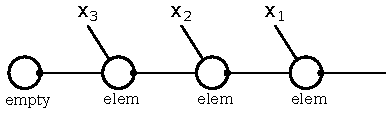
\includegraphics[width=0.7\linewidth]{pictures/jun-19/drawing-processes}
		\caption{Visualization of the processes (circles) involved in implementing a queue}
		\label{fig:drawing-processes}
	\end{figure}
	
	
	The type of \(elem\) reflects that it uses a stored value \(x\) of type \(A\) and a ``tail'' queue \(t\), its interface it that of \(queue_A\). So, we have:
	\[ x:A, t:queue_A \vdash elem :: (q:queue_A) \]
	
	The implementation is shown below, the blue text at the end of each line indicates the type we have at the moment. 
	\begin{align*}
		q \leftarrow elem \leftarrow t,x = \textsc{case } q 
		&(enQ \Rightarrow 
		&y \leftarrow \textsc{recv } q; 
		&& {\color{blue} (x:A, t:queue_A \vdash q:A \multimap queue_A)}\\
		&                 &t.enQ;  
		&& {\color{blue}\qquad (x:A,t:queue_A,y:A\vdash q:queue_A)}\\
		&                 &\textsc{send }t,y;  
		&& {\color{blue}(x:A,y:A,t:A \multimap queue_A\vdash q:queue_A)}\\
		&                 & q \leftarrow elem \leftarrow t,x
		&& {\color{blue}(x:A,t:queue_A\vdash q:queue_A)}\\[1.5em]
		&| deQ \Rightarrow 
		& q.some; 
		&& {\color{blue} (x:A, t:queue_A \vdash q:A \otimes queue_A)}\\
		&& \textsc{send }q,x ; 
		&& {\color{blue} (x:A, t:queue_A \vdash q:queue_A)}\\
		&& q \leftarrow t)
		&& {\color{blue} (t:queue_A \vdash q:queue_A)}
		\end{align*}
		
		
	Empty has the following type
	\[ \vdash elem :: (q:queue_A) \]

	The implementation is shown below again:
		\begin{align*}
	q \leftarrow empty = \textsc{case } q 
	&(enQ \Rightarrow 
	&y \leftarrow \textsc{recv } q; 
	&& {\color{blue} (\vdash q:A \multimap queue_A)}\\
	&                 &e \leftarrow empty;  
	&& {\color{blue}\qquad (y:A\vdash q:queue_A)}\\
	&                 & q \leftarrow elem \leftarrow e,y
	&& {\color{blue}(x:A,e:queue_A\vdash q:queue_A)}\\[1.5em]
	&| deQ \Rightarrow 
	& q.none; 
	&& \\
	&& \textsc{close }q 
	&& {\color{blue} (\vdash q:1)}
	\end{align*}
	
	
	\subsubsection{Other related advances}
	\begin{itemize}
		\item Shared memeory instead of message passing
		\item parallel complexity $\longrightarrow$ temporal logic (ICFP'18)
		\item sequential complexity
	\end{itemize}
	
	
	%----------------------------------------------------------------------------------------
	% BIBLIOGRAPHY
	%----------------------------------------------------------------------------------------
	
	\bibliographystyle{apalike}
	
	\bibliography{sample}
	
	%----------------------------------------------------------------------------------------
	
	
\end{document}